\flushleft{\section{Interpolación (1D)}}

\newtheorem*{mydeff}{Definición}
\begin{mydeff}
La función $y=P(x)$ $``$interpola$"$   los datos $(x_{1},y_{1})$,...,$(x_{n},y_{n})$  si $P(x_{i}) = y_{i}$ para cada $i=1,...,n$
\end{mydeff}

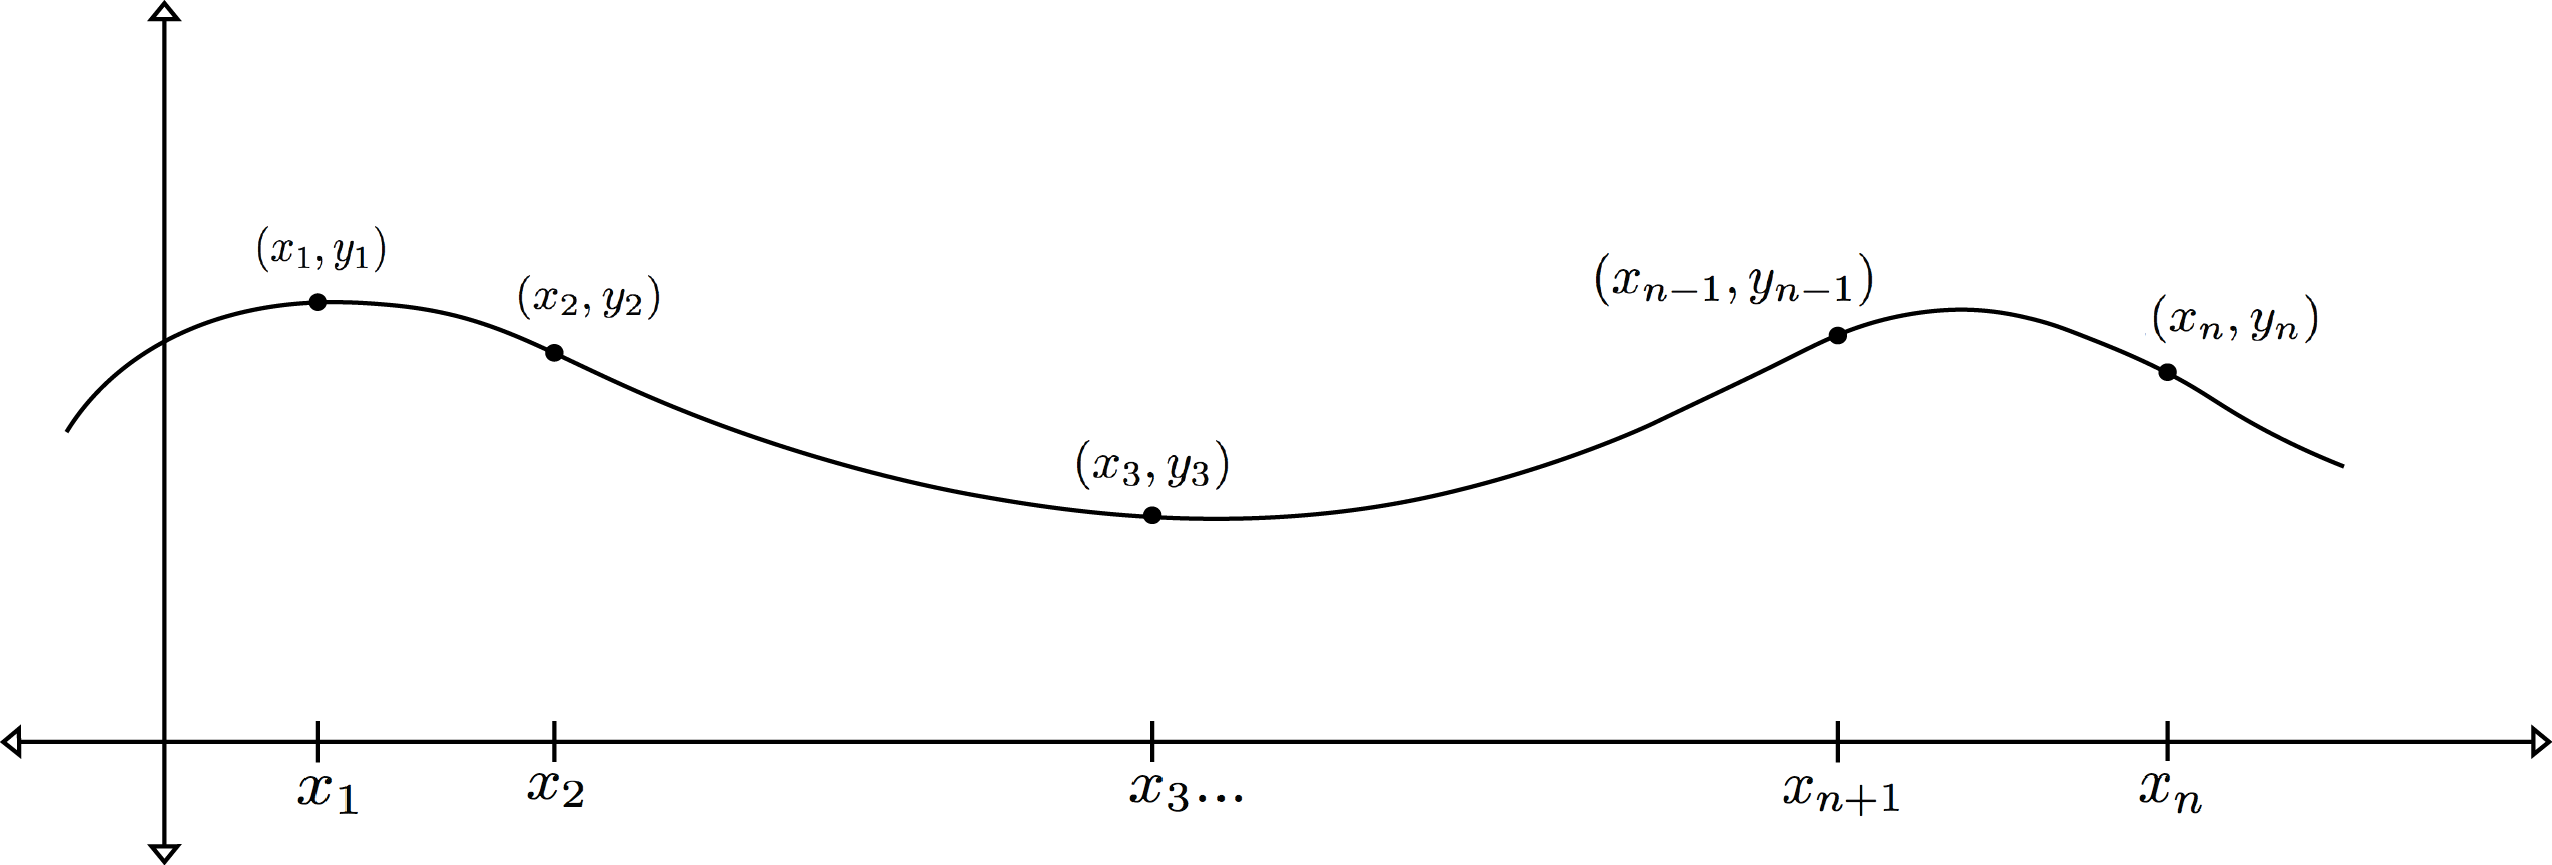
\includegraphics[scale=0.75]{seccion9/graficos/G1-1.png}

\subparagraph{Ejemplo}

¿Cuál es el polinomio de grado mínimo que interpola $(x_{1},y_{1})$ y $(x_{2},y_{2})$?\\

\begin{tabular}{cc|c}
& & \hspace*{3cm} lineal o cuadrático o etc... \\
\scalebox{0.8} % Change this value to rescale the drawing.
{
\begin{pspicture}(0,-3.5578125)(9.473437,3.5378125)
\psline[linewidth=0.04](1.6534375,3.5178125)(1.6534375,-2.8821876)(8.453438,-2.8821876)(8.473437,-2.9021876)
\psline[linewidth=0.04](8.453438,-2.8821876)(9.453438,-2.8821876)(9.453438,-2.8821876)
\psline[linewidth=0.04](1.6534375,3.5178125)(1.4534374,3.3178124)(1.6534375,3.5178125)(1.8534375,3.3178124)(1.8534375,3.3178124)
\psline[linewidth=0.04](9.253437,-2.6821876)(9.453438,-2.8821876)(9.253437,-3.0821874)(9.453438,-2.8821876)
\psline[linewidth=0.04](1.4534374,-0.6821875)(1.8534375,-0.6821875)(1.8734375,-0.7021875)
\psline[linewidth=0.04](1.4534374,1.5178125)(1.8534375,1.5178125)(1.8734375,1.4978125)
\psline[linewidth=0.04](4.2534375,-2.6821876)(4.2534375,-3.0821874)(4.2534375,-3.0821874)
\psline[linewidth=0.04](6.8534374,-2.6821876)(6.8534374,-3.0821874)(6.8734374,-3.1021874)
\usefont{T1}{ppl}{m}{n}
\rput(0.61875,1.5128125){\footnotesize $Y_{2}$}
\usefont{T1}{ppl}{m}{n}
\rput(0.69875,-0.6871875){\footnotesize $Y_{1}$}
\usefont{T1}{ppl}{m}{n}
\rput(4.25875,-3.3271875){\footnotesize $X_{1}$}
\usefont{T1}{ppl}{m}{n}
\rput(6.87875,-3.3471875){\footnotesize $X_{2}$}
\end{pspicture} 
}  & &\\
& &\\
& & \\
\end{tabular}


\newpage
%----------------------------------------------------------------------------------------------------------------------------------------------------------------




\subsection{Matriz de Vandermonde}
\begin{align*}
\left(\begin{array}{cc}
1 & x_{1} \\ 1 & x_{2}
\end{array}\right)
\left(\begin{array}{cc}
a_{0} \\ a_{1}
\end{array}\right)
=
\left(\begin{array}{cc}
y_{1} \\ y_{2}
\end{array}\right)
\end{align*} 

\begin{align*}
\left(\begin{array}{ccc}
1 & x_{1} & x^2_{1} \\ 1 & x_{2} & x^2_{2} \\ 1 & x_{3} & x^2_{3}
\end{array}\right)
\left(\begin{array}{cc}
a_{0} \\ a_{1} \\ a_{2}
\end{array}\right)
=
\left(\begin{array}{cc}
y_{1} \\ y_{2} \\ y_{3}
\end{array}\right)
\end{align*}

\underline{Recuerde:}
\begin{align*}
 \frac{||x-\tilde{x}||}{||x||} \leq K(A) \cdot \frac{||b-A \cdot \tilde{x} ||}{|| b ||}
\end{align*}

\subsection{Interpolación de Lagrange} 
\begin{equation*}
 \begin{split}
  P_{n-1}(x) & =y_{1} \cdot L_{1}(x)+...+y_{n} \cdot L_{n}(x) \\
 & = \sum_{i=1}^{n} y_{i} \cdot L_{i}(x) \\
 \text{donde } \ \ \ \ & L_{i}(x_{i})=1, \ \ \ L_{i}(x_{J})=0 \ \ \ \ \text{ para } i\neq J \\
 \end{split}
\end{equation*}
Ejemplo: 
\begin{align*}
 P_{n-1}(x_{J}) & =y_{1}:L_{1}(x_{J})+...+y_{J} \cdot L_{J}(x_{J})+...+y_{n} \cdot L_{n}(x_{J}) \\
 & =y_{1} \cdot 0+...+ \underline{y_{J}} \cdot 1+...+y_{n} \cdot 0 \\
 P_{n-1}(x_{J}) & =y_{J}
\end{align*}
\newpage


%----------------------------------------------------------------------------------------------------------------------------------------------------------------


 

 \underline{Ejemplo}: 

\begin{tabular}{lrr}
\multirow{4}{5cm}{\scalebox{0.65}{
\begin{pspicture}(0,-2.6864061)(7.0921874,2.6864061)
\psline[linewidth=0.04cm](1.63,2.1585937)(1.63,-2.0414062)
\psline[linewidth=0.04cm](1.63,-2.0414062)(6.63,-2.0414062)
\psline[linewidth=0.04cm](1.63,2.1585937)(1.43,1.9585937)
\psline[linewidth=0.04cm](1.63,2.1585937)(1.83,1.9585937)
\psline[linewidth=0.04cm](6.63,-2.0414062)(6.43,-1.8414062)
\psline[linewidth=0.04cm](6.63,-2.0414062)(6.43,-2.2414062)
\psline[linewidth=0.04cm](1.45,1.1385938)(1.85,1.1385938)
\psline[linewidth=0.04cm](2.63,-1.8414062)(2.63,-2.2414062)
\psline[linewidth=0.04cm](5.23,-1.8414062)(5.23,-2.2414062)
\usefont{T1}{ppl}{m}{n}
\rput(2.7145312,-2.4314063){\large $x_{1}$}
\usefont{T1}{ppl}{m}{n}
\rput(5.3545313,-2.4514062){\large $x_{2}$}
\psline[linewidth=0.04cm](1.45,-0.86140627)(1.85,-0.86140627)
\usefont{T1}{ppl}{m}{n}
\rput(0.69453126,1.1485938){\large $y_{2}$}
\usefont{T1}{ppl}{m}{n}
\rput(0.69453126,-0.8514063){\large $y_{1}$}
\psdots[dotsize=0.12](2.63,-0.82140625)
\psdots[dotsize=0.12](5.21,1.1585938)
\psdots[dotsize=0.12](2.63,-0.8414062)
\psline[linewidth=0.04cm](2.63,-0.8414062)(5.23,1.1585938)
\usefont{T1}{ppl}{m}{n}
\rput(1.6345313,2.4985938){\small Y}
\usefont{T1}{ppl}{m}{n}
\rput(6.936094,-2.0614061){\small X}
\end{pspicture} 
}
}
 & \multicolumn{2}{p{5cm}}%
 {\centering $P_{1}(x)= y_{1} \cdot L_{1}(x) + y_{2} \cdot L_{2}$ \\}\tabularnewline 
 & \multicolumn{1}{p{3cm}}%
{\centering $L_{1}(x)= \frac{(x - x_{2})}{(x_{1} - x_{2})}$}
 & \multicolumn{1}{p{1.7cm}}%
{ \scalebox{0.65}{
\begin{pspicture}(0,-2.6657813)(5.93375,2.6657813)
\psline[linewidth=0.04cm](0.4915625,2.1979687)(0.4915625,-2.0020313)
\psline[linewidth=0.04cm](0.4915625,-2.0020313)(5.4915624,-2.0020313)
\psline[linewidth=0.04cm](0.4915625,2.1979687)(0.2915625,1.9979688)
\psline[linewidth=0.04cm](0.4915625,2.1979687)(0.6915625,1.9979688)
\psline[linewidth=0.04cm](5.4915624,-2.0020313)(5.2915626,-1.8020313)
\psline[linewidth=0.04cm](5.4915624,-2.0020313)(5.2915626,-2.2020311)
\psline[linewidth=0.04cm](0.3115625,0.79796875)(0.7115625,0.79796875)
\psline[linewidth=0.04cm](1.4915625,-1.8020313)(1.4915625,-2.2020311)
\psline[linewidth=0.04cm](4.0915623,-1.8020313)(4.0915623,-2.2020311)
\usefont{T1}{ppl}{m}{n}
\rput(0.04703125,0.8329688){\large 1}
\usefont{T1}{ppl}{m}{n}
\rput(1.765,-2.3670313){\large $x_{1}$}
\usefont{T1}{ppl}{m}{n}
\rput(4.405,-2.3870313){\large $x_{2}$}
\usefont{T1}{ppl}{m}{n}
\rput(0.49609375,2.4779687){\small Y}
\usefont{T1}{ppl}{m}{n}
\rput(5.777656,-2.0220313){\small X}
\end{pspicture} 
}
}
 \tabularnewline 
  & $L_{2}(x)= \frac{(x - x_{2})}{(x_{2} - x_{1})}$   & \scalebox{0.65}{
\begin{pspicture}(0,-2.6657813)(5.93375,2.6657813)
\psline[linewidth=0.04cm](0.4915625,2.1979687)(0.4915625,-2.0020313)
\psline[linewidth=0.04cm](0.4915625,-2.0020313)(5.4915624,-2.0020313)
\psline[linewidth=0.04cm](0.4915625,2.1979687)(0.2915625,1.9979688)
\psline[linewidth=0.04cm](0.4915625,2.1979687)(0.6915625,1.9979688)
\psline[linewidth=0.04cm](5.4915624,-2.0020313)(5.2915626,-1.8020313)
\psline[linewidth=0.04cm](5.4915624,-2.0020313)(5.2915626,-2.2020311)
\psline[linewidth=0.04cm](0.3115625,0.79796875)(0.7115625,0.79796875)
\psline[linewidth=0.04cm](1.4915625,-1.8020313)(1.4915625,-2.2020311)
\psline[linewidth=0.04cm](4.0915623,-1.8020313)(4.0915623,-2.2020311)
\usefont{T1}{ppl}{m}{n}
\rput(0.04703125,0.8329688){\large 1}
\usefont{T1}{ppl}{m}{n}
\rput(1.765,-2.3670313){\large $x_{1}$}
\usefont{T1}{ppl}{m}{n}
\rput(4.405,-2.3870313){\large $x_{2}$}
\usefont{T1}{ppl}{m}{n}
\rput(0.49609375,2.4779687){\small Y}
\usefont{T1}{ppl}{m}{n}
\rput(5.777656,-2.0220313){\small X}
\end{pspicture} 
} \\
\end{tabular}



  
\begin{align*}
 P_{1}(x) & = y_{1} \cdot \frac{x-x_{2}}{x_{1} - x_{2}} + y_{2} \cdot \frac{(x - x_{2})}{(x_{2} - x_{1})} \\
 &= a_{0} + a_{1}x \ \ \text{(similar a la ``Matriz de vandermonde'')} \\
 &= \underbrace{\left[  \frac{y_{1} \cdot (-x_{2}) }{(x_{1} - x_{2})} + \frac{y_{2} \cdot (-x_{1})}{(x_{2} - x_{1})} \right]}_{a_{0}} +\underbrace{\left[  \frac{y_{1} }{(x_{1} - x_{2})} + \frac{y_{2} }{(x_{2} - x_{1})} \right]}_{a_{1}} \cdot x \\
 \end{align*}     
 \hrulefill
 
Para $\underline {\overline{X}} = \lbrace x_{1},...,x_{n} \rbrace$ \\


\begin{tabular}{lr}
$L_{k}(x) = \frac{l_{k}(x)}{l_{k}(x_{k})}$ & 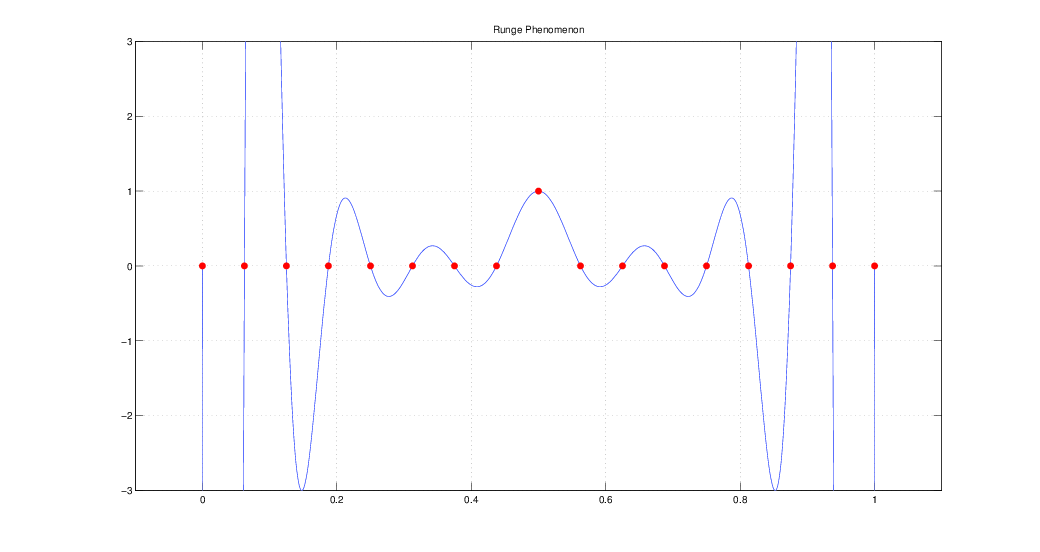
\includegraphics[scale=0.25]{seccion9/graficos/G3-4.png}
\end{tabular}


\begin{align*}
L_{k}(x) = \frac{(x-x_{1})(x - x_{2})...(x- x_{k-1})(x - x_{k+1})...(x - x_{n})}{(x_{k} -x_{1})(x_{k} - x_{2})...(x_{k}- x_{k-1})(x_{k} - x_{k+1})...(x_{k} - x_{n})}
\end{align*}



%----------------------------------------------------------------------------------------------------------------------------------------------------------------


\newpage

donde 
\begin{align*}
 (x&-x_{1})(x - x_{2})...(x- x_{k-1})(x - x_{k+1})...(x - x_{n}) \\
 &\updownarrow\\
 l_{k}(x) = \prod_{i=1,i \neq k}^{n}  (x & -x_{i}), L_{k}(x)= \frac{l_{k}(x)}{l_{k}(x_{k})}
\end{align*}
 \hrulefill
 
\newtheorem*{thm}{Teorema}
\begin{thm}
Sea $(x_{1},y_{1}),...,(x_{n},y_{n})$ $``$n$"$  puntos en el plano con \underline{distinto} $``\underline{x_{i}}''$. entonces existe uno y sólo un 
polinomio $P(x)$ de grado $n-1$ o $``$\underline{menor}$"$  que satisface
$$
P(x_{i}) = y_{i}, \ \ \text{para} \ \  i=1:n
$$
\end{thm}


\begin{tabular}{m{2cm} m{12cm}}
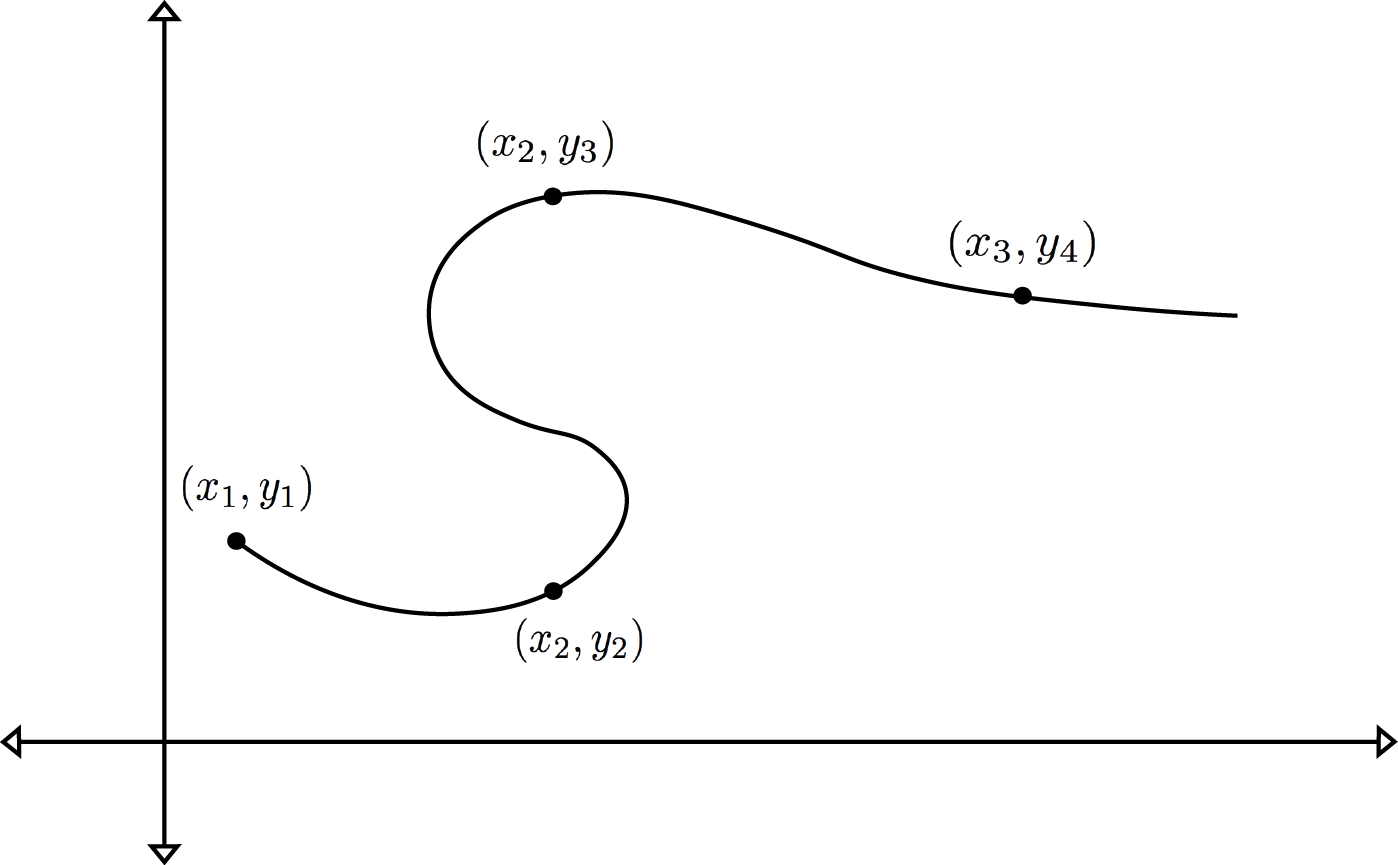
\includegraphics[scale=0.65]{seccion9/graficos/G4-1.png} & \hspace*{5cm} \begin{large}¿se puede?\end{large}  \\
\scalebox{0.7}{
\begin{pspicture}(0,-2.4101562)(9.951875,2.3901563)
\psline[linewidth=0.04cm](1.731875,2.3701563)(1.731875,-1.6298437)
\psline[linewidth=0.04cm](1.731875,-1.6298437)(9.931875,-1.6298437)
\psline[linewidth=0.04cm](9.931875,-1.6298437)(9.731875,-1.4298438)
\psline[linewidth=0.04cm](9.931875,-1.6298437)(9.731875,-1.8298438)
\psline[linewidth=0.04cm](1.731875,2.3701563)(1.531875,2.1701562)
\psline[linewidth=0.04cm](1.731875,2.3701563)(1.931875,2.1701562)
\psline[linewidth=0.04cm](1.531875,0.37015626)(1.931875,0.37015626)
\psline[linewidth=0.04cm](3.331875,-1.4298438)(3.331875,-1.8298438)
\psline[linewidth=0.04cm](4.931875,-1.4298438)(4.931875,-1.8298438)
\psline[linewidth=0.04cm](6.531875,-1.4298438)(6.531875,-1.8298438)
\psline[linewidth=0.04cm](8.131875,-1.4298438)(8.131875,-1.8298438)
\usefont{T1}{ppl}{m}{n}
\rput(0.681875,0.39015624){\large $y_{0}$}
\usefont{T1}{ppl}{m}{n}
\rput(3.301875,-2.1498437){\large $x_{1}$}
\usefont{T1}{ppl}{m}{n}
\rput(4.881875,-2.1698437){\large $x_{2}$}
\usefont{T1}{ppl}{m}{n}
\rput(6.481875,-2.1698437){\large $x_{3}$}
\usefont{T1}{ppl}{m}{n}
\rput(8.101875,-2.1898437){\large $x_{4}$}
\psdots[dotsize=0.12](3.331875,0.37015626)
\psdots[dotsize=0.12](4.931875,0.37015626)
\psdots[dotsize=0.12](6.531875,0.37015626)
\psdots[dotsize=0.12](8.131875,0.37015626)
\psline[linewidth=0.04cm](3.331875,0.37015626)(8.131875,0.37015626)
\end{pspicture} 
} & \hspace*{5cm}$P_{n-1}(x) = \rule{40mm}{0.1mm}$ \\
\end{tabular}


Considerando 2 puntos:\\
\begin{align*}
P_{1}(x) &= y_{0} \cdot \frac{(x - x_{2})}{(x_{1} - x_{2})} + y_{0} \cdot \frac{(x - x_{1})}{(x_{2} - x_{1})} \\
&= y_{0} \cdot \left( \frac{x - x_{2}}{x_{1} - x_{2}} - \frac{x - x_{1}}{x_{1} - x_{2}} \right) \\
&= y_{0} \cdot \left(  \frac{x_{1} - x_{2}}{x_{1} - x_{2}}  \right) \\
&= \underline{y_{0}}
\end{align*}





%----------------------------------------------------------------------------------------------------------------------------------------------------------------



\newpage

\subsection{Diferencias divididas de Newton} 

\underline{Recuerde:}
\begin{align*}
 P(x)  = 1+2 \cdot x&+3 \cdot x^2 + 4 \cdot x^3 \\
  =1+x \cdot (&2+x \cdot (3+4 \cdot x)) \\
  &\uparrow\\
  \text{Mín} &\ \ \text{número de operaciones}\\
 P_{n-1}(x)  = &\sum_{i=0}^{n-1} a_{i} \cdot x^i \Leftrightarrow \text{ Matriz de Vandermonde} \\
 P_{n-1}(x)  = &\sum_{i=1}^{n} Y_{i} \cdot L_{i}(x)
\end{align*}
\underline{Def:}  Denotemos que \underline{$f[x_{1}, x_{2} ... x_{n-1} x_{n}]$} es el coeficiente del término $x^{n-1}$ en el único polinomio que interpola $(x_{i}, \underbrace{f(x_{i})}_{Y_{i}})$. 
\begin{align*}
 & , \ \ P_{n-1}(x)= \sum_{i=0}^{n-1} a_{i} x^i = a_{0} + a_{1} \cdot x +...+\underline{a_{n-1}} \cdot x^{n-1} \\
 \Rightarrow P_{n-1}(x) = f [x_{1}] & + f[x_{1} \ \ x_{2}] \cdot (x-x_{1}) \\ 
 & +f[x_{1} \ \ x_{2} \ \ x_{3}] \cdot (x-x_{1}) \cdot (x-x_{2}) \\
 & \ \ \ \ \vdots \\
 & + f[x_{1} ... x_{n}] \cdot (x-x_{1}) ... (x-x_{n-1})
\end{align*}
\underline{Ej:} \ \ \ \ $(x_{1}, y_{1}), (x_{2}, y_{2}), (x_{3}, y_{3})$\\[2\baselineskip]
\begin{center}
\begin{tabular}{|c|c|c|}
\hline
$x_{1}$ & $y_{1} $ & $ \displaystyle = f[x_{1}]$ \\
\hline 
$x_{2}$ & $y_{2}$  & $= f[x_{2}]$ \\ 
\hline 
$x_{3}$ & $y_{3}$  & $= f[x_{3}]$\\
\hline 
\end{tabular} 
\hspace*{-0.19cm}
\begin{tabular}{|c|}
\hline
$ \displaystyle f[x_{1} \ \ x_{2}]=   \frac{f[x_{2}] - f[x_{1}]}{x_{2}-x_{1}}$ \\
\hline
$ \displaystyle f[x_{2} \ \ x_{3}] = \frac{f[x_{3}] - f[x_{2}]}{x_{3}-x_{2}}$\\
\hline
\end{tabular}
\hspace*{-0.19cm}
\begin{tabular}{|c|}
\hline
$ \displaystyle f[x_{1} \ \ x_{2} \ \ x_{3}] = \frac{f[x_{2} \ \  x_{3}] - f[x_{1} \ \  x_{2}]}{x_{3} - x_{1}}$ \\
\hline
\end{tabular}
\vspace*{0.5cm} \\
 $\Rightarrow P_{2}(x)=f[x_{1}]+f[x_{1} \ \ x_{2}] \cdot (x-x_{1})+f[x_{1} \ \ x_{2} \ \ x_{3}] \cdot (x-x_{1}) \cdot (x-x_{2})$
\end{center}


%----------------------------------------------------------------------------------------------------------------------------------------------------------------


\newpage
\section*{Algorítmicamente}
Input: $\underline {\overline{X}} = [x_{1}, x_{2}, ..., x_{n}], \ \ \underline {\overline{Y}} =[y_{1}, ..., y_{n}]$\\
Code:\\
\begin{algorithmic}[1]
\FOR {$J =1: n $}
\STATE {$f[x_{J}]= \underline {\overline{Y}}_{J} $}
\ENDFOR
\FOR{$i= 2:n$}
\FOR{$J= 1: n+1- i$}
\STATE{$\displaystyle f[x_{J}...x_{J+i-1}] = \frac{f[x_{J+1} ... x_{J+i-1}] - f[x_{J}... x_{J+i-2}]}{x_{J+i-1}-x_{J}}$}
\ENDFOR
\ENDFOR
\end{algorithmic}


\rule{150mm}{0.1mm} \\
\begin{align*}
 P_{n-1}(x) = \sum_{i=1}^{n} f[x_{1} ... x_{i}] \cdot \prod_{J=1}^{i-1} (x-x_{J}) \\
\end{align*}
\rule{150mm}{0.1mm}\\[2\baselineskip]
\underline{Ej:} \ \ \ \ $(0,1), (2,3), (3,0)$ \\[2\baselineskip]
\begin{tabular}{cc|c}
$\underline{Lagrange}:$ &$ P_{2}(x) =  y_{1} \cdot L_{1}(x) + y_{2} \cdot L_{2}(x)+ y_{3} \cdot L_{3}(x)$ & $\underline{Vandermonde}:$ \\
& & \\
& $L_{1}(x )= \displaystyle \frac{(x-2)(x-3)}{(0-2)(0-3)}$& $P_{2}(x) = a_{0} + a_{1} \cdot x + a_{2} \cdot x^{2}$\\
 & $\begin{array}{c}
 L_{2}(x)= \displaystyle \frac{(x-0)(x-3)}{(2-0)(2-3)}\\
 L_{3}(x) = \displaystyle \frac{(x-0)(x-2)}{(3-0)(3-2)}
 \end{array}$ 
 & $\left( \begin{matrix} 1&0 &0 \\ 1 & 2 & 4  \\ 1 & 3 & 9 \end{matrix} \right)$
 $ \left( \begin{matrix} a_{0} \\ a_{1}  \\ a_{2} \end{matrix} \right) = $
 $ \left( \begin{matrix} 1 \\ 3  \\ 0 \end{matrix} \right) $\\
& $ \displaystyle P_{2}(x) = 1\cdot \frac{(x-2)(x-3)}{6}+ 3 \cdot \frac{(x) \cdot(x-3)}{-2} + 0 \cdot L_{3}(x)$ &\\
&$ \displaystyle = 1 + \frac{11}{3} \cdot x - \frac{4}{3} \cdot x^{2} = a_{0} + a_{1} \cdot x + a_{2} \cdot x^{2} $ &
\end{tabular}

\underline{D.D.Newton }\\[2\baselineskip]
\begin{tabular}{|c|c|}
\hline 
0 &  1 \\
\hline 
2 & 3  \\ 
\hline 
3 & 0  \\ 
\hline 
\end{tabular} 
\hspace*{-0.19cm}
\begin{tabular}{|c|}
\hline 
1 \\
\hline 
-3 \\
\hline  
\end{tabular}
\hspace*{-0.19cm}
\begin{tabular}{|c|}
\hline 
$ \displaystyle \frac{-4}{3}$ \\
\hline  
\end{tabular}
$\Rightarrow$
\begin{tabular}{cc}
$P_{2}(x)$ &$= 1 + 1 \cdot (x-0) + (\frac{-4}{3}) \cdot (x-0)(x-2)$  \\
\end{tabular} \\
\begin{center}
¿Qué hago si quiero agregar 1 punto nuevo?
\end{center}


%----------------------------------------------------------------------------------------------------------------------------------------------------------------
\newpage


\underline{D.D Newton}:\\[2\baselineskip]
\begin{tabular}{cc}
$x_{i}$ & \hspace*{-0.2cm}$y_{i}$ \\
\end{tabular}\\
\begin{tabular}{|c|c|}
\hline 
0 &  1 \\
\hline 
2 & 3  \\ 
\hline 
3 & 0  \\ 
\hline
1 & 0  \\
\hline 
\end{tabular} 
\hspace*{-0.19cm}
\begin{tabular}{|c|}
\hline 
1 \\
\hline 
-3 \\
\hline 
0 \\
\hline 
\end{tabular}
\hspace*{-0.19cm}
\begin{tabular}{|c|}
\hline 
$\frac{-4}{3}$ \\
\hline 
$\frac{3}{-1}$ \\
\hline 
\end{tabular}
\hspace*{-0.19cm}
\begin{tabular}{|c|}
\hline
$\frac{-5}{3}$ \\
\hline
\end{tabular}\ \
\begin{tabular}{cc}
$\displaystyle P_{3}(x)$ &$= P_{2}(x) + (\frac{-5}{3}) \cdot (x-0)(x-2)\cdot(x-3)$  \\
 & $ \displaystyle = 1+1 \cdot (x-0)- \frac{4}{3}(x-0)(x-2)$ \\
 & \ \ \ \ \ \ \ \ \ \ \ $ \displaystyle \frac{-5}{3} \cdot (x-0)(x-2)(x-3)$
\end{tabular} \\[4\baselineskip]



\underline{Ejemplo}: \underline{3.7}
$$
f(x) = \sin(x), \text{4 puntos equiespaciados en} \left[0, \frac{\pi}{2}\right]
$$
\\
\begin{python}
import matplotlib.pyplot as plt
import numpy as np
import matplotlib.patches as mpatches

x = np.linspace(0, np.pi/2, 200)
fig = plt.figure(figsize=(10,7), dpi=80)
ax = fig.add_subplot(111)
ax.set_title(' f(x) = sin(x)',fontsize=18)

plt.plot(x, np.sin(x))
plt.xlabel('x [rad]')
plt.ylabel('sin(x)')
plt.xlim(0, np.pi/2)
plt.ylim(0, 1)
plt.grid()
t1 = 0
t2 = np.pi/6
t3 = np.pi/3
t4 = np.pi/2

red_patch = mpatches.Patch(color='blue', label='sin(x)')
plt.legend(bbox_to_anchor=(1, 0.95),handles=[red_patch])

plt.scatter([t1],[np.sin(t1)], 20, color ='blue')
plt.scatter([t2],[np.sin(t2)], 20, color ='blue')
plt.scatter([t3],[np.sin(t3)], 20, color ='blue')
plt.scatter([t4],[np.sin(t4)], 20, color ='blue')

plt.scatter([t1],0, 20, color ='red')
plt.scatter([t2],0, 20, color ='red')
plt.scatter([t3],0, 20, color ='red')
plt.scatter([t4],0, 20, color ='red')
plt.xticks([0,np.pi/6,np.pi/3, np.pi/2],
       [r'$0$',r'$+\pi/6$',r'$+\pi/3$', r'$+\pi/2$'])

plt.yticks([0, +0.5, +0.86602, +1],
       [r'$0$',r'$+0.5$',r'$+0.86602$', r'$+1$'])

plt.savefig('seccion9/graficos/fig2.pdf', format='pdf')
print(r"""
\begin{figure}[htbp]
    \centering
    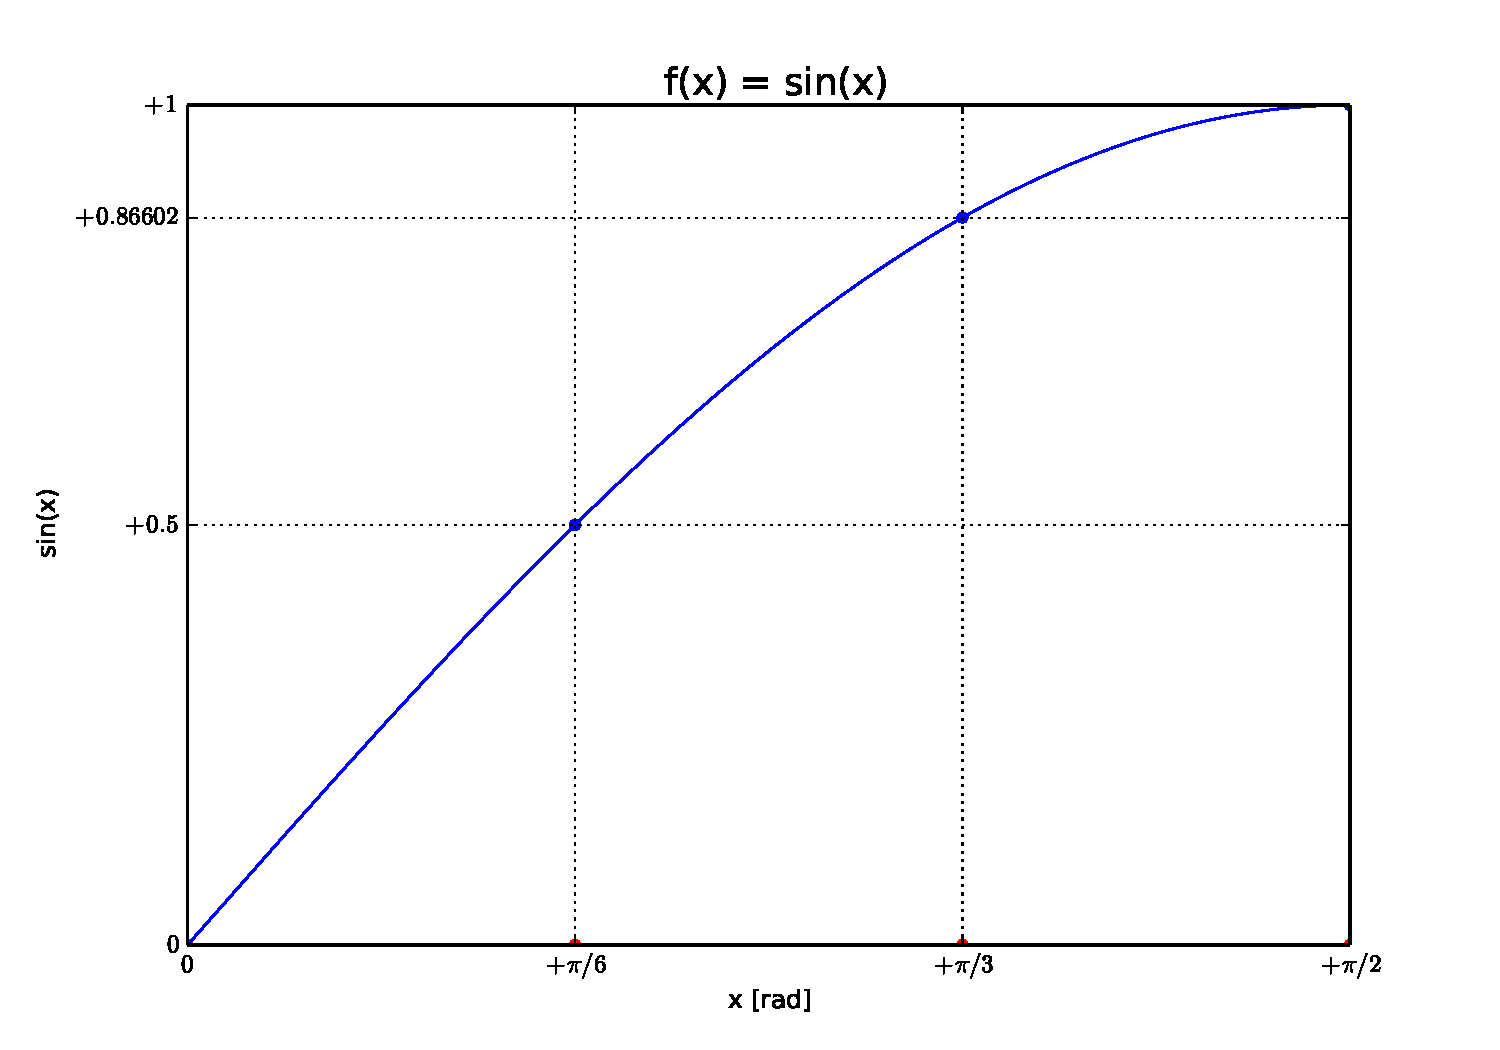
\includegraphics[width=8cm]{seccion9/graficos/fig2.pdf}
    \label{fig:comparison}
\end{figure}
""")
\end{python}
\\
\begin{tabular}{cc}
$x_{i}$ &  \ \ \ \ \ $y_{i} $
\end{tabular}\\
\begin{tabular}{|c|c|}
\hline 0 & 0\\
\hline
$\displaystyle \frac{\pi}{6}$& $\frac{1}{2}$ \\
\hline
$\displaystyle \frac{2 \pi}{6}$&0.8660 \\
\hline
$ \displaystyle \frac{\pi}{2}$& 1 \\
\hline
\end{tabular}
\hspace*{-0.19cm}
\begin{tabular}{|c|}
\hline
0.9549 \\
\hline
0.6990 \\
\hline
0.2259\\
\hline
\end{tabular}
\hspace*{-0.19cm}
\begin{tabular}{|c|}
\hline
-0.2443 \\
\hline
-0.4232 \\
\hline
\end{tabular}
\hspace*{-0.19cm}
\begin{tabular}{|c|}
\hline
-0.1139 \\
\hline
\end{tabular}\\
\begin{tabular}{cc}
\ \  $\uparrow$ &\ \ \ \ \ $\uparrow$
\end{tabular}\\
\hspace*{0.6cm} data 
\begin{align*}
\Rightarrow P_{3}(x) = 0 + 0.9549 \cdot (x&-0) -0.2443 \cdot (x) \cdot \left(x - \frac{\pi}{6}\right) \\
&-0.1139 \cdot (x-0)\left(x - \frac{\pi}{6}\right)\left(x - \frac{2 \pi}{6}\right)
\end{align*}
%----------------------------------------------------------------------------------------------------------------------------------------------------------------

\newpage


\subsection{Error de Interpolación}

\underline{Th:} \ \ Asuma que $P(x)$ es el polinomio interpolador (de grado $n-1$ o menor) que ajusta $n$ puntos $(x_{1}, \ \ y_{1}), ..., (x_{n}, \ \ y_{n})$. El error de interpolación es \\
\begin{center}
 \begin{align*}
  f(x) - P(x) = \frac{(x-x_{1})(x-x_{2})...(x-x_{n})}{n!} \cdot f^{(n)}(c)
 \end{align*}
\end{center}
\ \ \ \ \ \ \ donde $c$ está entre el menor y el mayor de los números $x, x_{1}, ... , x_{n}$.\\[2\baselineskip]

\underline{Recuerde:} \ \ $f(x)=f(x_{0})+f'(x_{0}) \cdot (x-x_{0})+ ... + \frac{f^{(n)}(c)}{n!} \cdot (x-x_{0})^n$ \\[2\baselineskip]

\begin{center}
 ¿Qué tan buena es la interpolación de $f(x)$ obtenida por $P(x)$? 
 \vspace*{1cm}
\end{center}
$
\begin{array}{ll}
Error(x) = |f(x) - P(x)| \ \ \ \ \Rightarrow \text{Peor caso} = & \max |f(x)-P(x)| \\
 \vspace*{-0.5cm} & \\
 &  \hspace{0.2cm} x\\
\end{array}
$
$
\begin{array}{ll}
\Rightarrow \max Error = & \max |(x-x_{1})...(x-x_{n})| \cdot \displaystyle \frac{|f^{(n)}(c)|}{n!}  \\
 \vspace*{-0.5cm} & \\
 &  \hspace{0.2cm} x\\
\end{array}
$\\[3\baselineskip]
Ver ejemplo 3.7 en Matlab. \\
 \begin{center}
  \underline{Runge Phenomenon} \ \ $\Leftarrow$ Muy Importante\\
  Ver en Matlab.
 \end{center}
\newpage

\subsection{Interpolación de Chebyshev} 

 \subparagraph{Motivación:} ¿Qué podemos mejorar de la fórmula de error de interpolación?\\[2\baselineskip]
 \subparagraph{Recuerde:} \ \ \ \ \ \ \ \ \begin{Large} $\frac{(x-x_{1}) \cdot (x-x_{2}) ... (x-x_{n})}{n!} \cdot f^{(n)} (c) $ \end{Large}\\[2\baselineskip]
 Consideremos \ \ \ \ $x=[-1, 1] $ \\
 \begin{center}
  ¿Podemos encontrar $ x_{1}, ..., x_{n}$ de tal forma que $(x-x_{1})...(x-x_{n})$ es minimizado?\\
  \vspace*{1cm}
  \rule{60mm}{0.1mm}
 \end{center}
\subparagraph{Ej:} Consideremos \ \ \ \ n$=2$, \\
\begin{center} 
$
\begin{array}{lll}
 \Rightarrow& (x-x_{1}) \cdot (x-&x_{2})  \\
\Rightarrow&   w(x_{1}, x_{2}) = & \max |(x-x_{1}) \cdot (x-x_{2})|  \\
 \vspace*{-0.5cm} & &\\
 & &   $\begin{small}$x \in [-1,1]$\end{small}$
\end{array}
$
\end{center}
\hspace*{2cm} \fbox{\parbox[c]{5cm}{$[x_{1}, x_{2}]=   \arg \min w(x_{1}, x_{2})$ \begin{center} $x_{1}, x_{2} \in [-1,1]$ \end{center}}} \\
\begin{center}
 ¿Cómo obtenemos $x_{1}, x_{2}$ ? \\
 \vspace*{3cm}
¿Y en general $x_{1}, ..., x_{n}$?\\
\vspace*{1cm}
\end{center}
 
 %----------------------------------------------------------------------------------------------------------------------------------------------------------------

\newpage


\newtheorem*{thm2}{Teorema}
\begin{thm}
La elección de los números reales $-1 \leq x_{1},...,x_{n} \leq 1$ que hace el valor de \\
\begin{align*}
\max_{-1 \leq x \leq 1} |(x-x_{1})...(x-x_{n})|
\end{align*}\\
lo más pequeño posible es
\end{thm}
$
\begin{array}{lcl}
\text{raíces} & \hspace{2cm}  & \\
\text{de los} & \rightarrow &$\begin{large} $x_{i} = \cos \left( \frac{(2 \cdot i -1) \cdot \pi}{2 \cdot n}\right), \ i=1,...,n$  \end{large}$\\
\text{polinomios} & & \\
\text{de Chebyshev} & & \\
\end{array}$\\
\hspace*{1.5cm} \begin{tabular}{|c}
 \\
 \hspace*{1cm} y el valor mínimo es \begin{LARGE}$\frac{1}{2^{n-1}}$\end{LARGE}
 \\
 ~\\
 \hspace*{1cm} De hecho, el mínimo es \\
 \\
 \hspace{1.5cm} \begin{Large}$(x-x_{1})...(x - x_{n}) = \frac{1}{2^{n-1}} \cdot T_{n}(x)$\end{Large}
 \\
 ~\\
 ~\\
\end{tabular}\\
\hspace*{1.5cm} $\longrightarrow$ donde $T_{n}(x) = \cos (n \cdot \arccos(x))$ es el $n$-ésimo polinomio de Chebyshev \\

\underline{Nota}: \begin{align*}
T_{n+1}(x) &= 2 \cdot x \cdot T_{n}(x) - T_{n-1}(x) \\
T_{0}(x) &= 1 \\
T_{1}(x) &= x \\
T_{2}(x) &= 2 \cdot x^{2} -1 \\
\ \ \vdots 
\end{align*}




 %----------------------------------------------------------------------------------------------------------------------------------------------------------------

\newpage


\begin{center} ¿Cuál es la interpretación gráfica?\\ \end{center}
\begin{align*}
x_{i} = \cos(\theta_{i}), \ \ \ \theta_{i} = \frac{(2i - 1)\cdot \pi}{2n}, \ \ \ i=1,...,n
\end{align*}
\begin{large}
\begin{tabular}{cc|c}
$i=1   \Rightarrow \theta_{1} = \frac{\pi}{2n}$ &\hspace{2cm} & $\theta_{1} - \theta = \frac{1}{n} \cdot \frac{\pi}{2} = \frac{1}{5} \cdot \frac{\pi}{2} $ \\
& &\\
$n = 5  \Rightarrow \theta_{1} = \frac{1}{5} \cdot \frac{\pi}{2}$& \hspace{2.5cm}& $\theta_{i+1} - \theta_{i} = \frac{2}{n} \cdot \frac{\pi}{2} = \frac{\pi}{5}$ \\
& & \\
$\theta_{2} = \frac{3 \pi}{2n} = \frac{3 \pi}{10},$ & $ \theta_{3} = \frac{5 \pi}{2 \cdot 5} = \frac{\pi}{2}$ & \\
& &\\
$\theta_{4} = \frac{7 \pi}{2 \cdot 5} = \frac{7 \pi}{10},$ & $ \theta_{5} = \frac{9 \pi}{10}$ &
\end{tabular}
\end{large}
\begin{align*}
\Rightarrow x_{i} = \cos( \theta_{i})& \\
x_{1}= 0.9511, & x_{2}= 0.5878, x_{3}= 0.0000, x_{4}= -0.5878, x_{5}= -0.9511\\
\end{align*}

\begin{python}
import numpy as np
import matplotlib.pyplot as plt
import matplotlib.patches as mpatches

def filled_arc(center, radius, theta1, theta2, ax, color):

    circ = mpatches.Wedge(center, radius, theta1, theta2, fill=False, color=color)
    pt1 = (radius * (np.cos(theta1*np.pi/180.)) + center[0],
           radius * (np.sin(theta1*np.pi/180.)) + center[1])
    pt2 = (radius * (np.cos(theta2*np.pi/180.)) + center[0],
           radius * (np.sin(theta2*np.pi/180.)) + center[1])
    pt3 = center
    pol = mpatches.Polygon([pt1, pt2, pt3], color=ax.get_axis_bgcolor(),
                           ec=ax.get_axis_bgcolor(), lw=2 )
    ax.add_patch(circ)
    ax.add_patch(pol)

def Chebyshev(n,ax=None):
    x = [np.cos(((2*i-1)*np.pi)/(2*n)) for i in range(1,n+1)]
    y = [np.sin(((2*i-1)*np.pi)/(2*n)) for i in range(1,n+1)]
    if ax == None:
        return np.array(x)
    ax.set_ylim(-0.1,1.1)
    ax.set_xlim(-1.1,1.1)
    ax.plot(np.cos(np.linspace(0,np.pi)),np.sin(np.linspace(0,np.pi)),'k-')
    ax.plot([-2,2],[0,0],'k-')
    ax.plot([0,0],[-1,2],'k-')
    for i in range(len(y)):
        ax.plot([x[i],x[i]],[0,y[i]],'r-')
        ax.plot([0,x[i]],[0,y[i]],'r-')
        ax.annotate(str("%.4f" % x[i]), xy=(x[i], -0.07), xytext=(x[i], -0.07))
            
    ax.plot(x,[0]*len(x),'ro')
    ax.set_xlabel('x')
    ax.set_ylabel('y')
    ax.plot(x,y,'ro')
    
    filled_arc((0,0), 0.8, 0, 180-18 , ax1, "black")
    ax.text(-0.55, 0.4, r"$\theta_5$", fontsize=25)

    filled_arc((0,0), 0.7, 0, 180-54 , ax1, "black")
    ax.text(-0.17, 0.53, r"$\theta_4$", fontsize=25)

    filled_arc((0,0), 0.6, 0, 90 , ax1, "black")
    ax.text(0.12, 0.43, r"$\theta_3$", fontsize=25)

    filled_arc((0,0), 0.5, 0, 54 , ax1, "black")
    ax.text(0.3, 0.23, r"$\theta_2$", fontsize=25)

    filled_arc((0,0), 0.4, 0, 18, ax1, "black")
    ax.text(0.28, 0.015, r"$\theta_5$", fontsize=25)

    plt.savefig('seccion9/graficos/fig3.pdf', format='pdf')
    print(r"""
    \begin{figure}[htbp]
       \centering
        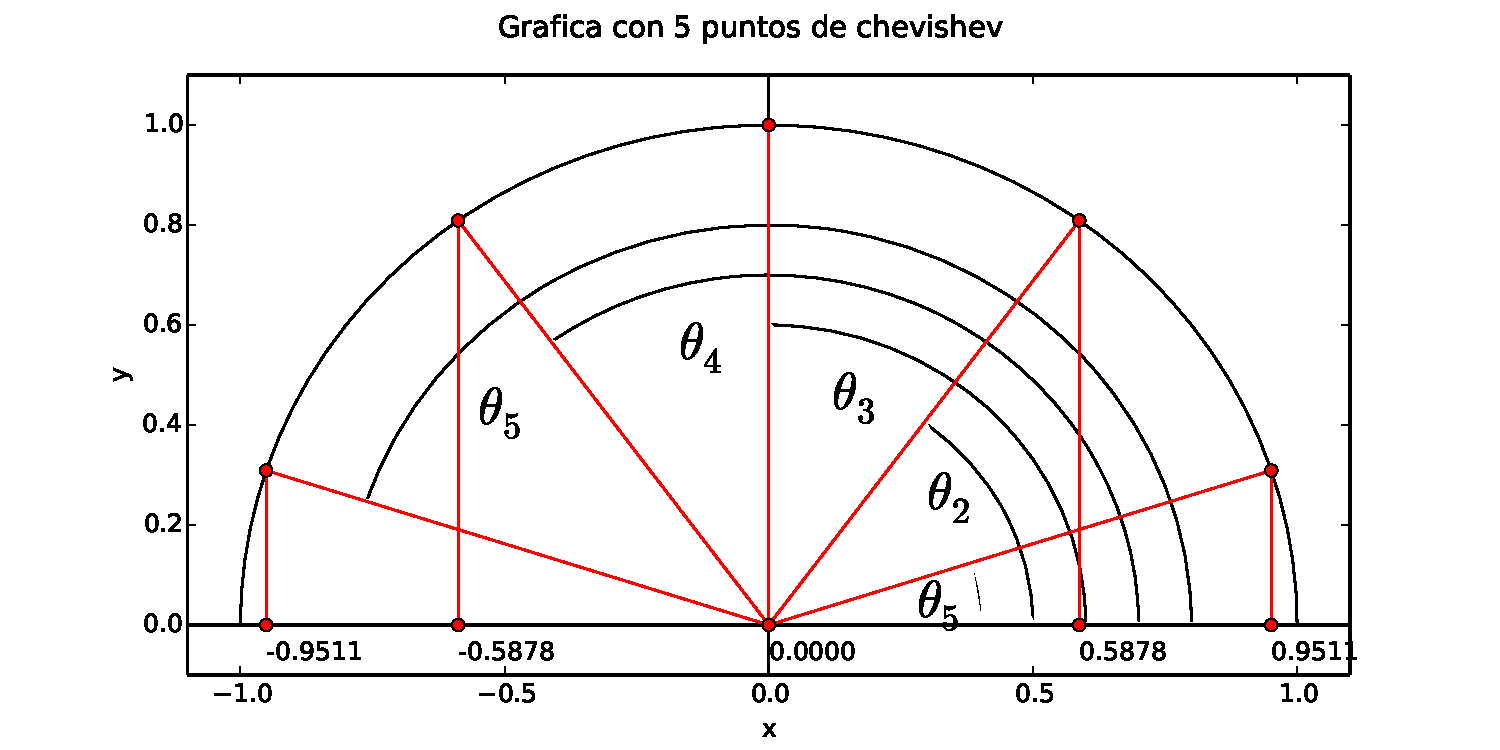
\includegraphics[width=18cm]{seccion9/graficos/fig3.pdf}
        \label{fig:comparison}
    \end{figure}
    """)
   

f, (ax1) = plt.subplots(1, figsize=(10,5))
f.suptitle('Grafica con 5 puntos de chevishev', fontsize=14)
Chebyshev(5,ax1)
\end{python}


%----------------------------------------------------------------------------------------------------------------------------------------------------------------

\newpage

Recuerde: $ W(x) = \prod_{i=1}^{n} (x - x_{i}) $\\[2\baselineskip]

\begin{center}
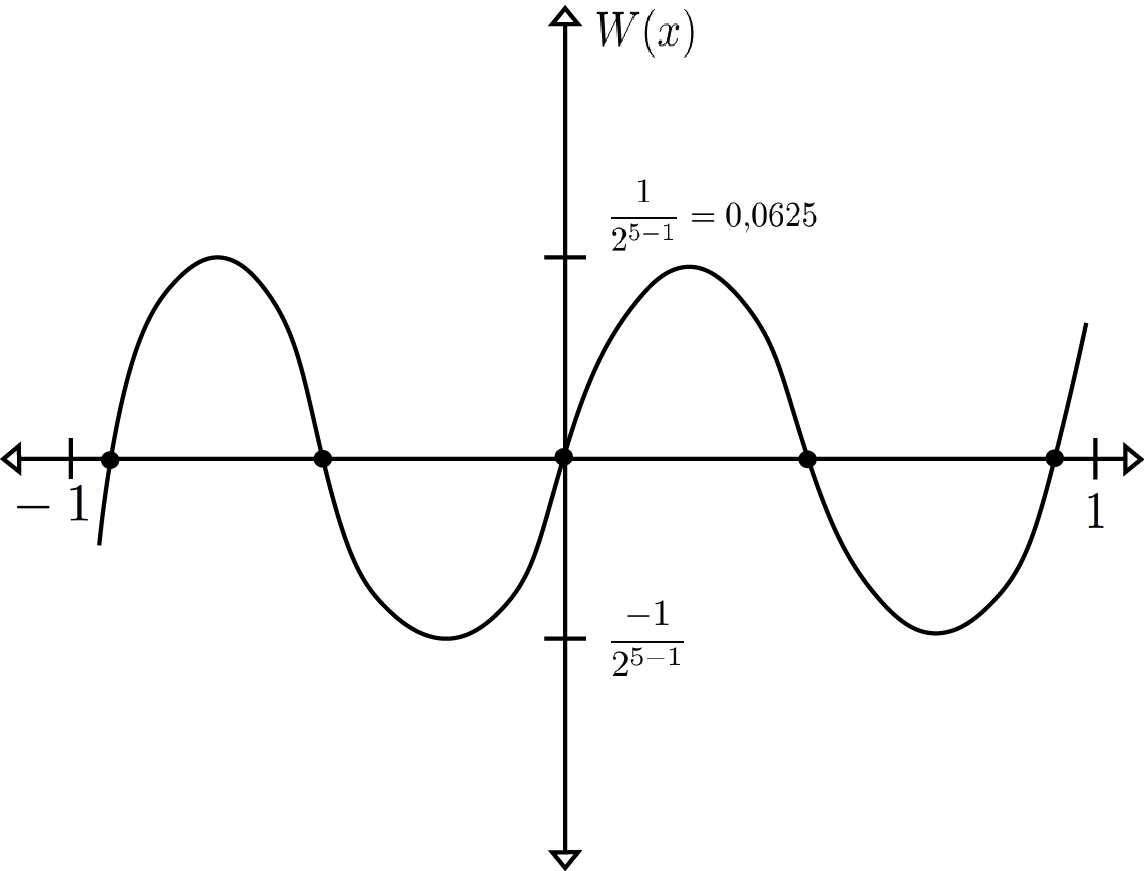
\includegraphics[scale=0.8]{seccion9/graficos/G12-1.png}
\end{center}

\underline{Ejemplo}: Ejemplo 3.10, Encuentre el peor caso del error para la diferencia de $e^{x}$ y el polinomio de Chebyshev de grado 4 en el intervalo $x = [-1,1]$.\\[2\baselineskip]
\hspace*{2.5cm} \\
\begin{align*}
\Rightarrow \hspace{2cm} |e^{x}-P_{4}(x)|=& \frac{|(x-x_{1})...(x-x_{5})|}{n!} \cdot |f^{(5)}(c)| \\
\\
 \leq & \frac{1}{2^{5-1}} \cdot \frac{1}{n!} |f^{(5)}(c)| \\
\\
f(x) =  e^{x} \Rightarrow f^{(5)}(c) = e^{x},& \text{max en} [-1,1] \Rightarrow e^{1}\\
\\
\Rightarrow \hspace{2cm} |e^{x} - P_{4}(x)| \leq & \frac{e}{2^{4} \cdot 5!} \approx 0.00142
\end{align*}



%----------------------------------------------------------------------------------------------------------------------------------------------------------------

\newpage
\subsection{Cambio de Variable}
\begin{center}
\vspace*{1cm}
 Chebyshev points: $-1 \leq x_{i} \leq 1$
 y en general $ f(x)$ definido en $a \leq x \leq b$ \\
\end{center}
 
$\Rightarrow$ \begin{tabular}{lrr}
\multirow{4}{6cm}{\scalebox{0.8} % Change this value to rescale the drawing.
{
\begin{pspicture}(0,-2.6639063)(5.93125,2.6639063)
\psline[linewidth=0.04cm](0.4890625,2.1560938)(0.4890625,-2.0439062)
\psline[linewidth=0.04cm](0.4890625,-2.0439062)(5.4890623,-2.0439062)
\psline[linewidth=0.04cm](0.4890625,2.1560938)(0.2890625,1.9560938)
\psline[linewidth=0.04cm](0.4890625,2.1560938)(0.6890625,1.9560938)
\psline[linewidth=0.04cm](5.4890623,-2.0439062)(5.2890625,-1.8439063)
\psline[linewidth=0.04cm](5.4890623,-2.0439062)(5.2890625,-2.2439063)
\psline[linewidth=0.04cm](0.3090625,1.1360937)(0.7090625,1.1360937)
\psline[linewidth=0.04cm](1.4890625,-1.8439063)(1.4890625,-2.2439063)
\psline[linewidth=0.04cm](4.0890627,-1.8439063)(4.0890627,-2.2439063)
\psline[linewidth=0.04cm](0.3090625,-0.86390626)(0.7090625,-0.86390626)
\psdots[dotsize=0.12](1.4890625,-0.82390624)
\psdots[dotsize=0.12](4.0690627,1.1560937)
\psdots[dotsize=0.12](1.4890625,-0.8439062)
\psline[linewidth=0.04cm](1.4890625,-0.8439062)(4.0890627,1.1560937)
\usefont{T1}{ppl}{m}{n}
\rput(0.0521875,1.1560937){\large b}
\usefont{T1}{ppl}{m}{n}
\rput(0.08765625,-0.8439062){\large a}
\usefont{T1}{ppl}{m}{n}
\rput(1.4332813,-2.5239062){\large -1}
\usefont{T1}{ppl}{m}{n}
\rput(4.0428123,-2.5239062){\large 1}
\usefont{T1}{ppl}{m}{n}
\rput(5.775156,-2.0639062){\large X}
\usefont{T1}{ppl}{m}{n}
\rput(0.45359376,2.4760938){\large Y}
\end{pspicture} 
}}
 & \multicolumn{2}{p{5cm}}%
 {\vspace*{2cm} }\tabularnewline 
 & \multicolumn{1}{p{3cm}}%
{ $ \displaystyle y = \displaystyle \frac{a+b}{2} + \displaystyle \frac{b-a}{2}\cdot x$ }
 & \multicolumn{1}{p{1.7cm}}%
{ }
 \tabularnewline 
  &   &  \\
\end{tabular}
 
 
\begin{tabular}{cc}
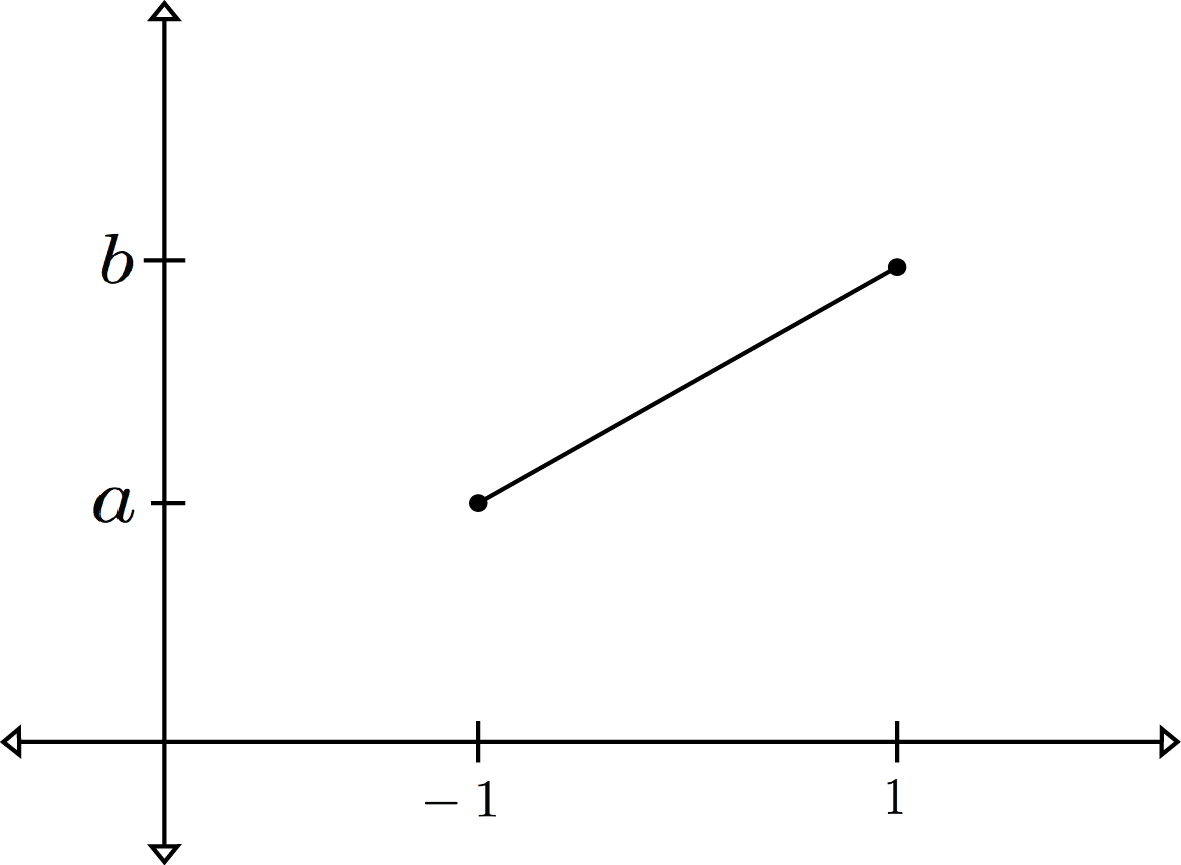
\includegraphics[scale=0.65]{seccion9/graficos/G13-1.png} & $y = \frac{a+b}{2} + \frac{b-a}{2}\cdot x$ \\
\end{tabular}

\vspace*{4cm}

$
\begin{array}{lll}
                
\Rightarrow &  \displaystyle \tilde{x}_{i}  = \displaystyle \frac{b+a}{2} + \displaystyle \frac{b-a}{2} \cdot & x_{i} \\
& \uparrow &  \uparrow \\
& \text{Chebyshev} & \text{Chebyshev points} \\
& \text{en} \ \ a \leq x \leq b & \text{en} \ \ -1 \leq x_{i} \leq 1 \\
& & \\ 
\end{array}$

$\Rightarrow  |(x-x_{i})...(x-x_{n})|  \leq \displaystyle \frac{(\frac{b-a}{2})^n}{2^{n-1}} \ \ \text{en} \ \ x=[a,b]   $                


\begin{center}
 También se podría hacer un cambio de variable de $[a,b]$ a $[-1,1]$ y usar la misma teoría.
\end{center}

\pagebreak
